\begin{recipe}
    [% 
        preparationtime = {\unit[10]{min}},
        portion = {\portion{2}},
        bakingtime = {\unit[15]{min}}
    ]
    {Broccoli pesto}

    \introduction{%
        My grandma who cooks only traditional food fell in love in this pesto.
        I can recommend it more!
    }
    \setRecipeLengths{
        ingredientswidth=5cm
    }
    \ingredients[13]{%
        1 & Broccoli with stem \\
        \unit[0.75]{c.} & Olive oil \\
        \unit[1]{c.} & Almonds\\
        1 & Onion\\
        2cm & Ginger\\
        3 & Garlic cloves\\
        \nicefrac{1}{2} bunch & Parsley \\
        \unit[5]{ts.} & \underline{Yeast flakes} \\
        & Chili \\
        & Nutmeg \\
        & Lemon juice 
    }

    \preparation{%
        \step Cut broccoli into pieces, cook on boiling water for 4-5 min.
        Drain and cool with cold water (preserve nice green colour).
        \step  To roast almonds (or any other seeds/nuts), preheat the frying pan well (the thicker the frying pan, the better (eg cast-iron)), do not add any fat.
        Keep it at high heat, stir from time to time (not too often, though!
        Let them roast).
        \step Dice ginger and onion, dice (or press) garlic.
        \step Blend everything. Voilà!
        \step  Serve with pasta, topped with cheese and cherry tomatoes. Or serve with bread. Or even with roast (as sauce) or raw vegetables (as dip).
    }

    \suggestion{%
       Instead of almonds, you can use sunflower seeds.
    }

    \hint{%
       When roasting seeds/nuts, remember to transfer them immediately to a bowl as the frying pan is still hot after turning the hob off.
    }

\end{recipe}

\begin{figure}[t]
    \centering
    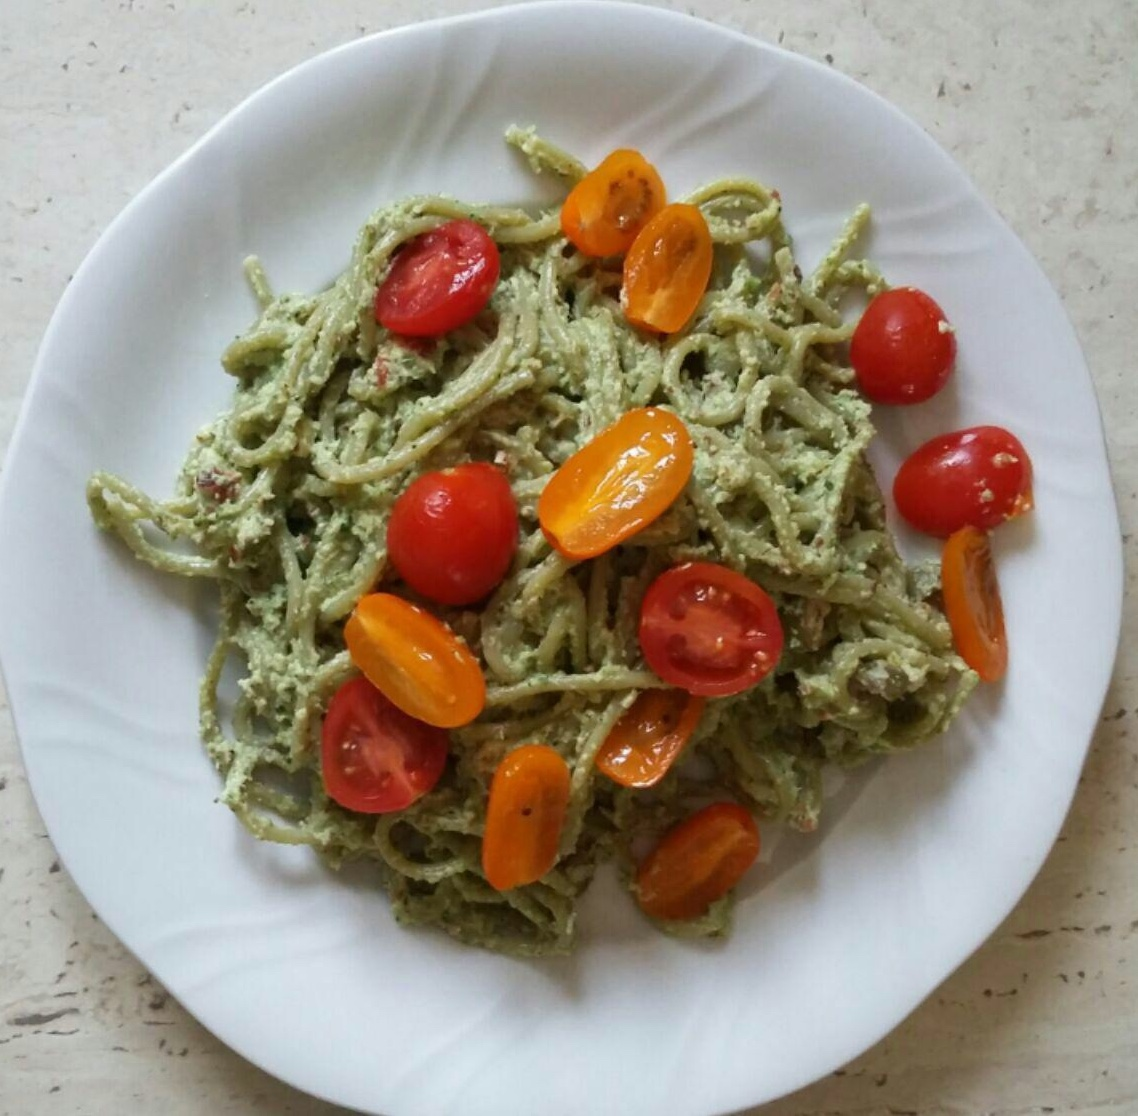
\includegraphics[width=12cm]{pic/brocolli_pesto}
\end{figure}
